\documentclass{article}
\usepackage[utf8]{inputenc}
\usepackage[T1]{fontenc}
\usepackage{graphicx}
\usepackage{hyperref}
\usepackage{xcolor}
\usepackage{amsmath, amssymb, amsthm}
\hypersetup{
    colorlinks=true,
    linkcolor=black,
    filecolor=magenta,      
    urlcolor=cyan,
    pdftitle={Overleaf Example},
    pdfpagemode=FullScreen,
    }
\title{Przewidywanie hałasu płatu lotniczego na podstawie obserwacji w tunelu aerodynamicznym (Airfoil Self-Noise)}
\author{Grzegorz Landowski i Rafał Kurek}
\begin{document}
\maketitle

\maketitle
\pagebreak
\tableofcontents
\pagebreak
\section{Co to jest sztuczna inteligencja?}

\textbf{Sztuczna inteligencja (ang. artificial intelligence - AI)} jest to próba zasymulowania przez maszynę pewnego zachowania, które wymaga inteligencji.\\
\break
Systemy AI mogą usprawniać swoje działania na podstawie zebranych informacji.\\
\break
Głównym celem sztucznej inteligencji jest naśladowanie ludzkiego sposobu postrzegania rzeczywistości i reagowania na nią, a następnie wykroczenie poza właściwe im ograniczenia.

\begin{figure}[h]
\caption{Schemat sztucznej inteligencji z raportu Game-changing technologies: Transformin production adn emplyment in Europe}
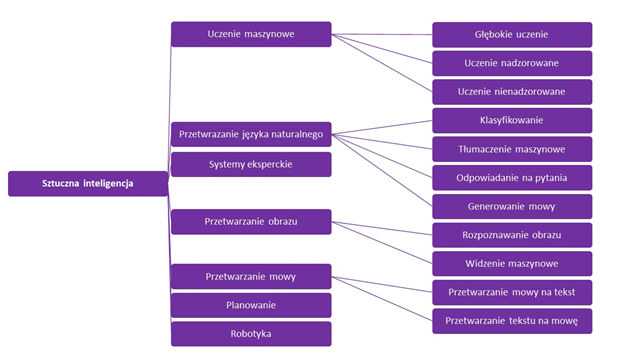
\includegraphics[scale=0.7]{schematsztucznejinteligencji}
\end{figure}

 Definicja sztucznej inteligencji z dokumentów Komisji Europejskiej brzmi:\\
\break
 "Systemy (…) zaprojektowane przez ludzi systemy oprogramowania (i ewentualnie również sprzętu), które, biorąc pod uwagę złożony cel, działają w wymiarze fizycznym lub cyfrowym, postrzegając swoje środowisko poprzez pozyskiwanie danych, interpretując zebrane ustrukturyzowane lub nieustrukturyzowane dane, rozumując na podstawie wiedzy lub przetwarzając informacje, uzyskane z tych danych i decydując o najlepszym działaniu (działaniach), jakie należy podjąć, aby osiągnąć dany cel. ".
\pagebreak

Organizacja Współpracy Gospodarczej i Rozwoju (OECD) także opracowała swoją definicję sztucznej inteligencji oraz jej schemat.\break
\\Według niej System AI to system oparty na koncepcji maszyny, która może wpływać na środowisko, formułując zalecenia, przewidywania lub decyzje dotyczące zadanego zestawu celów. Czyni to, wykorzystując dane wejściowe do:
\begin{itemize}
  \item postrzegania rzeczywistych lub wirtualnych środowisk
  \item streszczania takiego postrzegania w modele ręcznie lub automatycznie
  \item wykorzystywania interpretacji modeli do formułowania opcji wyników
\end{itemize}
\begin{figure}[h]
\caption{System AI według OECD}
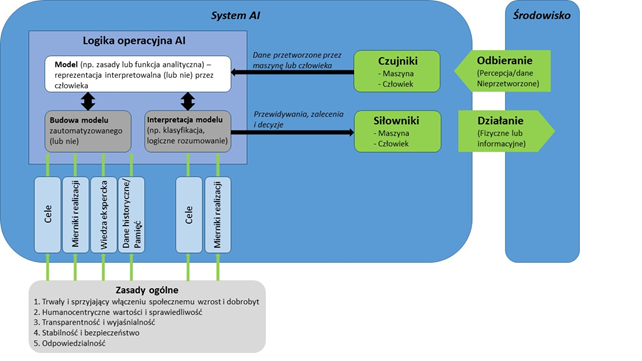
\includegraphics[scale=0.7]{systemai}
\end{figure}
Schemat systemu AI według OECD składa się z:
\begin{itemize}
  \item czujników (sensorów)
  \item logiki operacyjnej (modeli algorytmów)
  \item siłowników (aparatu wykonawczego)
\end{itemize}
Czujniki zbierają nieprzetworzone dane ze środowiska, a siłowniki podejmują działania w celu zmiany stanu środowiska. Kluczowa siła systemu sztucznej inteligencji znajduje się w jego logice operacyjnej (modelach algorytmów), która dla danego zestawu celów i na podstawie danych wejściowych z czujników zapewnia ekstrakcje (wynik) dla siłowników – jako zalecenia, przewidywania lub decyzje, które mogą wpłynąć na stan środowiska.
\pagebreak
\section{Uczenie maszynowe}
\textbf{Uczenie maszynowe (ang. machine learning)} to poddziedzina sztucznej inteligencji, które jest uogólnieniem algorytmów, które mają za zadanie w pewien sposób przetwarzać zbiór przykładów w celu realizacji określonego zadania. Podczas przetwarzania danych następują procesy uczenia i doskonalenia się, które nie są zaprogramowane. W uczeniu maszynowym algorytmy są trenowane pod kątem znajdowania wzorców i korelacji w dużych zbiorach danych oraz podejmowania najlepszych decyzji i formułowania prognoz na podstawie wyników takiej analizy.
\begin{figure}[h]
\caption{Schemat zależności między AI a uczeniem maszynowym}
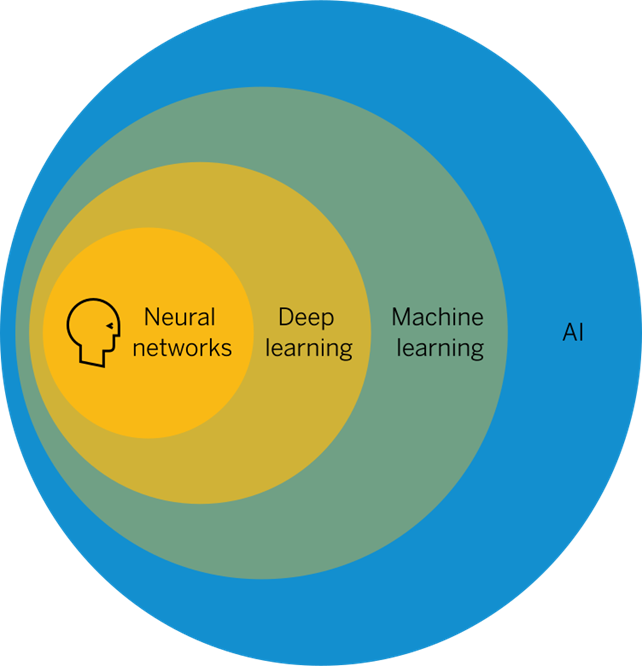
\includegraphics[scale=0.6]{AIauczeniemaszynowe}
\end{figure}
\\ 
Sztuczna inteligencja jest kategorią nadrzędną wobec wszystkich podzbiorów uczenia maszynowego. Pierwszy jej podzbiór stanowi uczenie maszynowe, kolejnym w jego obrębie jest głębokie uczenie, a wewnątrz niego znajdują się sieci neuronowe.
\pagebreak
\subsection{Sieci neuronowe}
Sieci neuronowe to podzbiór uczenia głębokiego. Składają się z neuronów, nazywanymi „węzłami”, które są pogrupowane w liczne warstwy, które działają równolegle. Kiedy neuron otrzymuje sygnał, przetwarza go i przekazuje tę informację do pozostałych neuronów, które są z nim połączone. Wzmocnienie neuronów umożliwia lepsze rozpoznawanie wzorców i uczenie się.
\break \\
W sieciach neuronowych wyróżnia się trzy typy warstw:
\begin{itemize}
  \item \textbf{warstwa wejściowa} – jej jedyną funkcją jest pobieranie danych i przekazywanie ich do pierwszej warstwy ukrytej.
  \item \textbf{warstwa ukryta} – warstwa odpowiedzialna za naukę i wykonywanie obliczeń, nie można do niej w sposób bezpośredni przekazywać informacji.
  \item \textbf{warstwa wyjściowa} – warstwa obliczająca wartości wyjściowe całej sieci i zwracająca je na zewnątrz.
\end{itemize}
\subsection{Uczenie głębokie}
Uczenie głębokie (ang. deep learning) jest poddziedziną uczenia maszynowego.
Podstawowym czynnikiem wyróżniającym uczenie głębokie od uczenia maszynowego jest to, że proces uczenia nie wymaga kontroli człowieka.
Może bazować na nieustrukturyzowanych danych w nieprzetworzonej formie (np. tekście, obrazach) i automatycznie określać zestaw cech, które rozróżniają kategorie danych.
Uczenie głębokie korzysta z sieci neuronowych uruchamiając wiele warstw sieci, uzyskując stopniowo wyniki na coraz wyższym poziomie dokładności.
\subsection{Metody uczenia maszynowego}
Dzieli się na:
\begin{itemize}
  \item \textbf{uczenie nadzorowane} - do uczenia algorytmów wykorzystuje zbiory danych z etykietami, które umożliwiają dokładne klasyfikowanie danych lub przewidywanie wyników. Zbiór uczący składający się z uporządkowanej pary i-tego obiektu i jego etykiety \[ X = \{x^{(i)},\ y^{(i)}\},\ gdzie\ i = 1...m\]
  \item \textbf{uczenie nienadzorowane} - wykorzystuje algorytmy uczenia maszynowego do analizowania i grupowania zbiorów danych bez etykiet. Algorytmy te wykrywają ukryte wzorce lub zgrupowania danych bez konieczności interwencji człowieka. Zbiór uczący składa się z i różnych obiektów \[X = \{ x^{(i)} \}\]
  \item \textbf{uczenie ze wzmocnieniem} - przykład uczenia maszynowego, w którym agent poprzez interakcję z otoczeniem uczy się pewnej polityki postępowania. Dostaje cel, który ma osiągnąć, ale nie wskazuję się mu drogi postępowania. Zawsze pożądane jest, aby każdy krok w algorytmie był podejmowany w celu osiągnięcia celu. W tego typu uczeniu algorytm uczy się poprzez mechanizm sprzężenia zwrotnego i doświadczenia z przeszłości. Za każdym razem, gdy ma zostać podjęty następny krok, otrzymuje informacje zwrotne z poprzedniego kroku, wraz z nauką z doświadczenia, aby przewidzieć, co może być następnym najlepszym krokiem. Drogą prób i błędów dąży do celu.
\begin{figure}[h]
\caption{mechanizm sprzężenia zwrotnego w uczeniu ze wzmocnieniem}
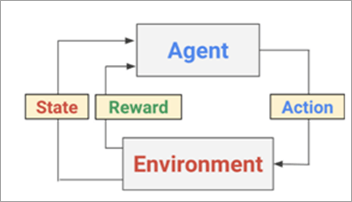
\includegraphics[scale=0.7]{uczenie_ze_wzmocnieniem}
\end{figure}
  
\end{itemize}
\section{Regresja liniowa}
Tematyka projektu opiera się o problem regresji. Regresja jest przykładem uczenia nadzorowannego i wyróżniamy:
\begin{itemize}
\item \textbf{regresję liniową}
\item \textbf{regresję logistyczną}
\end{itemize}
Do przewidzenia hałasu płatu lotniczego na podstawie obserwacji w tunelu aerodynamicznym korzystając ze zbioru danych "Airfoil Self-Noise" wykorzystaliśmy \textbf{regresję liniową} i to na jej opisie się skupimy.
\subsection{Wstęp do regresji liniowej}
Jak już zostało powiedziane regresja liniowa jest przykładem uczenia nadzorowanego.
\\
\\
W tym uczeniu mamy elementy uczące (cechy), które oznaczymy przez \textbf{\emph{x}}.
\\
\\
Z każdym elementem uczącym mamy związaną etykietę oznaczoną przez \textbf{\emph{y}}.
\\
\\
Przykładem nazywamy parę elementu uczącego oraz etykiety powiązanej z nią \textbf{\emph{(x, y)}}.
\\
\\
Mamy dany zbiór uczący składający się z \emph{m} przykładów oznaczony: \[X = \{x^{(i)},\ y^{(i)}\},\ gdzie\ i = 1...m\]
Każdy element uczący oraz jego etykieta jest numerowana poprzez indeks górny \textbf{\emph{i}}.
\\
\\
Element uczący $x^{(i)}$ możemy zakodować za pomocą wektora w n wymiarowej przestrzeni cech \[x^{(i)} \in R^n\]
Dla przykładu możemy opisać obiekt człowieka za pomocą dwóch cech (n=2) wzrostu i wagi.
\\
\\
Dla i-tego elementu uczącego możemy mieć tylko jedną etykietę $y^{(i)}$ (wyjście) albo też kilka etykiet (wyjść). Na przykład przy rozpoznawaniu typu pojazdu oprócz rozpoznania, że dany obiekt jest samolotem chcielibyśmy także rozpoznać jego kolor. W takim wypadku moglibyśmy zapisać, że nasza etykieta $y^{(i)}$ należy do iloczynu kartezjańskiego liczby możliwych wyjść i mozliwych różnych wartości tych wyjść:
\[y^{(i)} \in \{1...z\} \times \{1...\zeta\}\]
, gdzie z to liczba możliwych wyjść, a $\zeta$ to liczba możliwych parametrów każdego z tych wyjść.\newline
W takim przypadku mówilibyśmy o uczeniu multiklasowym, wieloetykietowym, gdzie z oznacza klasę, a $\zeta$ etykietę.
\\
\\
W uczeniu nadzorowanym wyjście może być:
\begin{itemize}
  \item \textbf{dyskretne} - tzn. może być przypisana klasa i wówczas problem nazywamy \textbf{klasyfikacją}.
  \item \textbf{wartością ciągłą} - wówczas problem nazywamy \textbf{regresją}, a wyjście może być opisane w \emph{Z} wymiarach:
  \[y^{(i)} \in R^Z\]
\end{itemize}
\subsection{Zadanie regresji liniowej}
Założenia:
\begin{itemize}
  \item$X \in \{x^{(i)}, y^{(i)}\},\ i=1...m$
  \item$x^{(i)} \in R^n$ i-ty element uczący jest określony w \emph{n} wymiarowej przestrzeni cech
  \item$y^{(i)} \in R$ i-te wyjście jest jednoelementową wartością, nieskalarną
\end{itemize}

Zadaniem regresji liniowej jest znalezienie takiej hipotezy (funkcji liniowej) $h_\Theta(x)$ , która opiszę nam możliwe jak najlepiej nasze dane uczące $\{x^{(i)}, y^{(i)}\}$.
\begin{figure}[h]
\caption{Przykładowa hipoteza $h_\Theta(x)$ opisująca dane uczące}
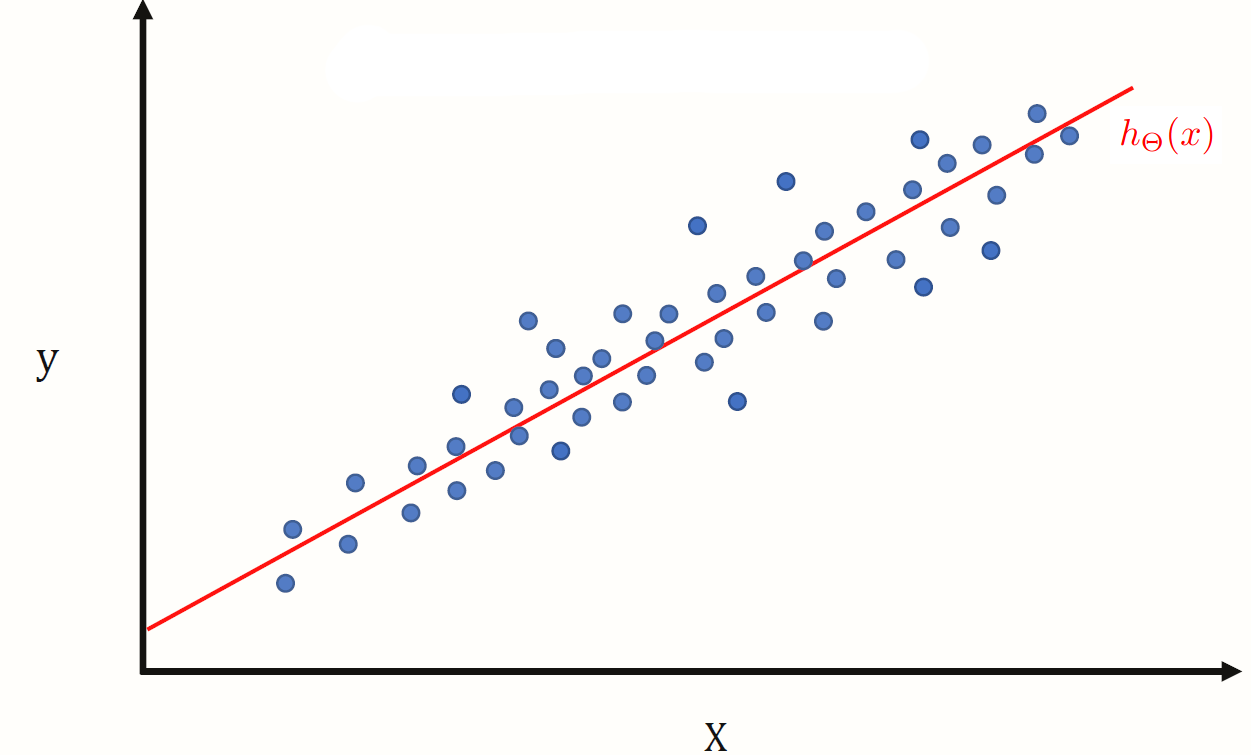
\includegraphics[scale=0.3]{linearRegression}
\end{figure}
\subsection{Cel regresji liniowej}
Celem regresji liniowej jest takie wytrenowanie zbioru uczącego, by uzyskać hipotezę $h_\Theta(x)$, która jak najlepiej opiszę dane uczące i za jej pomocą westymować (przewidzieć) wartości nowych danych uczących spoza pierwotnego zbioru uczącego \emph{X}.
\subsection{Dopasowywanie wzoru hipotezy}
Postać hipotezy, którą staramy się dopasować do danych uczących:
\[h_\Theta(x) = \Theta_0 + \Theta_1X\]
Wyznaczamy losową hipotezę i sprawdzamy jej odległość od punktów uczących. Wartość punktu i-tego to wartość rzeczywista, a wartość hipotezy w $x^{(i)}$ to estymacja\newline
Odległość i-tego punktu od wyznaczonej hipotezy nazywamy i-tym błędem i opisujemy danym wzorem:
\[e^{(i)} = {(h_\Theta(x^{(i)}) - y^{(i)})}^2 \]
Chcemy określić hipotezę za pomocą funkcji błędu danej wzorem:
\[J(\Theta) = \sum_{i} e^{(i)}\]
Parametry $\theta_i$ (zwane także wagami) parametryzują przestrzeń funkcji liniowych X $\rightarrow$ Y. To tych parametrów właśnie szukamy.\newline
Zapiszmy je w postaci wektorowej:
$\theta = \begin{bmatrix}
\Theta_0\\
\Theta_1
\end{bmatrix}$
\\
\\
Następnie możemy zapisać naszą hipotezę regresji liniowej w postaci wektorowej:
\[h_\Theta(x) = \Theta^Tx\]
Teraz należy znaleźć minimum funkcji błędu względem parametru $\Theta$:
\[\min_{\Theta}J(\Theta) = \min_{\Theta}\frac{1}{2}\sum_{i}e^{(i)} = \min_{\Theta}\frac{1}{2}\sum_{i=1}^m{(h_\Theta(x^{(i)})-y^{(i)})}^2\]
, pomnożenie sumy liczbą $\frac{1}{2}$ ułatwi dalsze obliczenia. Nie zmieni to współrzędnych, zmienią się tylko wartości bezwzględne błędów.
\\
\\
Chcemy znaleźć takie parametry, aby zminimalizować funkcję błędu. Zobaczmy czy zadziała następujący pomysł:

Zacznijmy od pewniej "odgadniętej" wartości początkowej. Następnie zmieniamy ją zgodnie z kierunkiem przeciwnym do gradientu funkcji błędu.

Gradient funkcji to wektor, którego kierunek pokrywa się z kierunkiem, w którym funkcja zmienia się najszybciej, a zwrot wskazuje kierunek, w którym funkcja rośnie. Formalnie jeden krok algorytmu minimalizacji gradientowej możemy zapisać:
\[\Theta_j \leftarrow\Theta_j - \eta\frac{\partial}{\partial\Theta_j}J(\Theta)\]
, gdzie parametr $\eta$ to współczynnik, który wpływa na wielkość kroków algorytmu.
\\
\\
Obliczamy pochodną $\frac{\partial}{\partial\Theta_i}J(\Theta)$:
\[\frac{\partial}{\partial\Theta_i}J(\Theta) = \frac{\partial}{\partial\Theta_i}\frac{1}{2}\sum_{i=1}^m{(h_\Theta(x^{(i)}) - y^{(i)})}^2 =
\frac{1}{2}\sum_{i=1}^m\frac{\partial}{\partial\Theta_i} {(h_\Theta(x^{(i)}) - y^{(i)})}^2 =
\]
\[
\frac{1}{2}\sum_{i=1}^m2(h_\Theta(x^{(i)}) - y^{(i)})\frac{\partial}{\partial\Theta_i}h_\Theta(x^{(i)}) =
\sum_{i=1}^m(h_\Theta(x^{(i)}) - y^{(i)})\frac{\partial}{\partial\Theta_j}\sum_{j=0}^n 0_j x_j^{(i)} =
\]
\[
\sum_{i=1}^m(h_\Theta(x^{(i)}) - y^{(i)})\sum_{j=0}^n\frac{\partial}{\partial\Theta_j} 0_j x_j^{(i)} =
\sum_{i=1}^m(h_\Theta(x^{(i)}) - y^{(i)})x^{(i)}_j
\]
\newpage
Posiadając wynik pochodnej można ropisać kroki postępowania:
\begin{itemize}
  \item Zainicjuj $\Theta_j$
  \item powtarzaj, aż zbiegniesz dla każdego $j:\Theta_j:= \Theta_j - \eta \sum_{i=1}^m(h_\Theta(x^{(i)}) - y^{(i)})x^{(i)}_j$
\end{itemize}

\section{Repozytorium GitHub z projektem}
Projekt w formacie Jupyter Notebook jest dostępny pod następującym linkiem \url{https://github.com/grzegorzlandowski/Airfoil-Self-Noise-regresja-liniowa.git}




\pagebreak

\section{Bibliografia}
\newcounter{boxlblcounter}  
\newcommand{\makeboxlabel}[1]{\fbox{#1.}\hfill}% \hfill fills the label box
\newenvironment{boxlabel}
  {\begin{list}
    {\arabic{boxlblcounter}}
    {\usecounter{boxlblcounter}
     \setlength{\labelwidth}{3em}
     \setlength{\labelsep}{0em}
     \setlength{\itemsep}{2pt}
     \setlength{\leftmargin}{1.5cm}
     \setlength{\rightmargin}{2cm}
     \setlength{\itemindent}{0em} 
     \let\makelabel=\makeboxlabel
    }
  }
{\end{list}}

\begin{boxlabel}
\item  \url{https://www.oracle.com/pl/artificial-intelligence/what-is-ai/}
\item  \url{https://www.gov.pl/web/ai/czym-jest-sztuczna-inteligencja2}
\item  \url{https://www.sap.com/poland/insights/what-is-machine-learning.html}
\item  \url{https://www.ibm.com/pl-pl/cloud/learn/machine-learning}
\item  \url{https://bulldogjob.pl/readme/czym-jest-deep-learning-i-sieci-neuronowe}
\item  \url{https://myservername.com/types-machine-learning}
\end{boxlabel}
\end{document}
